\documentclass{article}
\usepackage[utf8]{inputenc}
\usepackage{amsmath}
\usepackage{amsfonts}
\usepackage{amssymb}
\usepackage{graphicx}
\usepackage{geometry}
\usepackage{xcolor}
\usepackage{gensymb}
\usepackage{hyperref}
\usepackage{gensymb}
\usepackage{listings}

\newcommand{\inv}{^{-1}}   
\newcommand{\Z}{\mathbb Z}
\newcommand{\R}{\mathbb R}
\newcommand{\Q}{\mathbb Q}
\newcommand{\C}{\mathbb C}
\newcommand{\N}{\mathbb N}

\begin{document}

\newpage\noindent\textbf{1.}
\begin{center}
    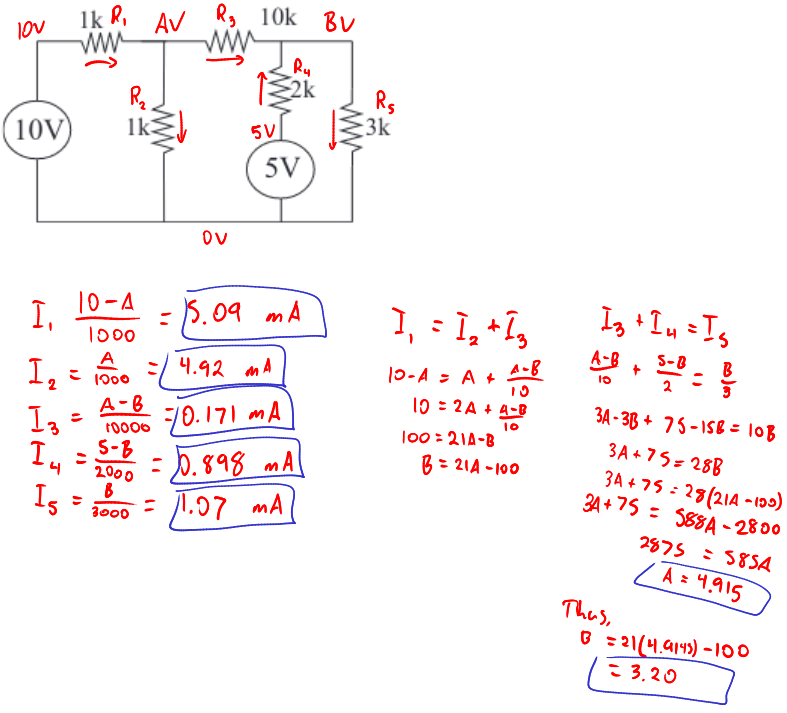
\includegraphics[scale=.7]{1.png}
\end{center}

\newpage\noindent\textbf{2.}
\begin{center}
    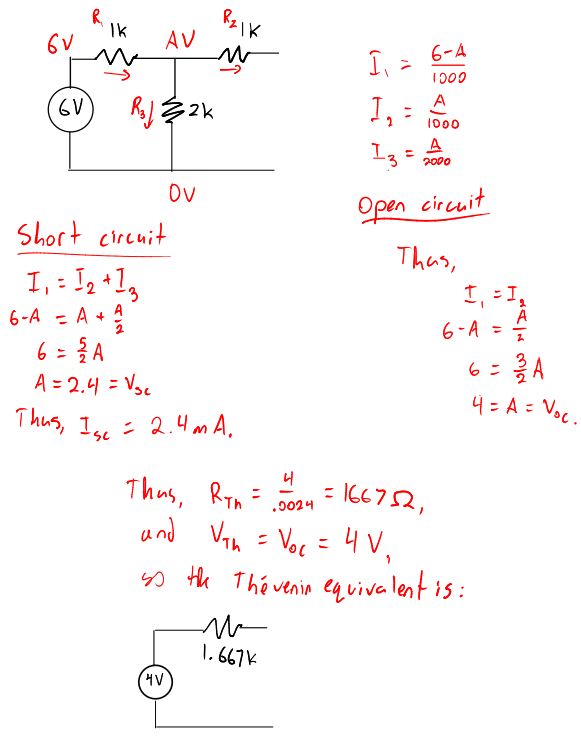
\includegraphics[scale=.7]{2.png}
\end{center}

\newpage\noindent\textbf{3.}

    When discharging begins, there is a high charge density on the negatively charged plate of the capacitor.
    Because of this, the repulsive force between electrons is high.
    As the magnitude of the charge on the plate decreases, the remaining electrons' collective repulsive force decreases, so the rate at which electrons leave the plate slows.

\newpage\noindent\textbf{4.}

    When the resistance of the variable resistor is high, then the voltage drop across it is large, so the output volume is low.
    Similarly, when the resistance is low, the voltage drop is small, so the output volume is high.
    The reason this works is that resistors provide a linear resistance, so the output wave is not distorted.

\newpage\noindent\textbf{5.}

    

\newpage\noindent\textbf{6.}

\newpage\noindent\textbf{7.}
        
\newpage\noindent\textbf{8.}

\newpage\noindent\textbf{9.}

\newpage\noindent\textbf{10.}


\end{document}
